\rewrite{falar sobre propostas baseada em chunks de exemplos}

\subsection{\emph{Framework Online-Offline} (FOO) para Agrupamento em FD} \label{ChAFD:framework}

Algoritmos de agrupamento baseados em exemplos podem ser resumidos em dois passos \cite{Cao2006,Yang2006}: abstração dos dados (componente\emph{online}) e agrupamento (componente \emph{offline}), ilustrados na \autoref{Fig:onlineOffline}.

\begin{figure}[!htb]
	\centering
	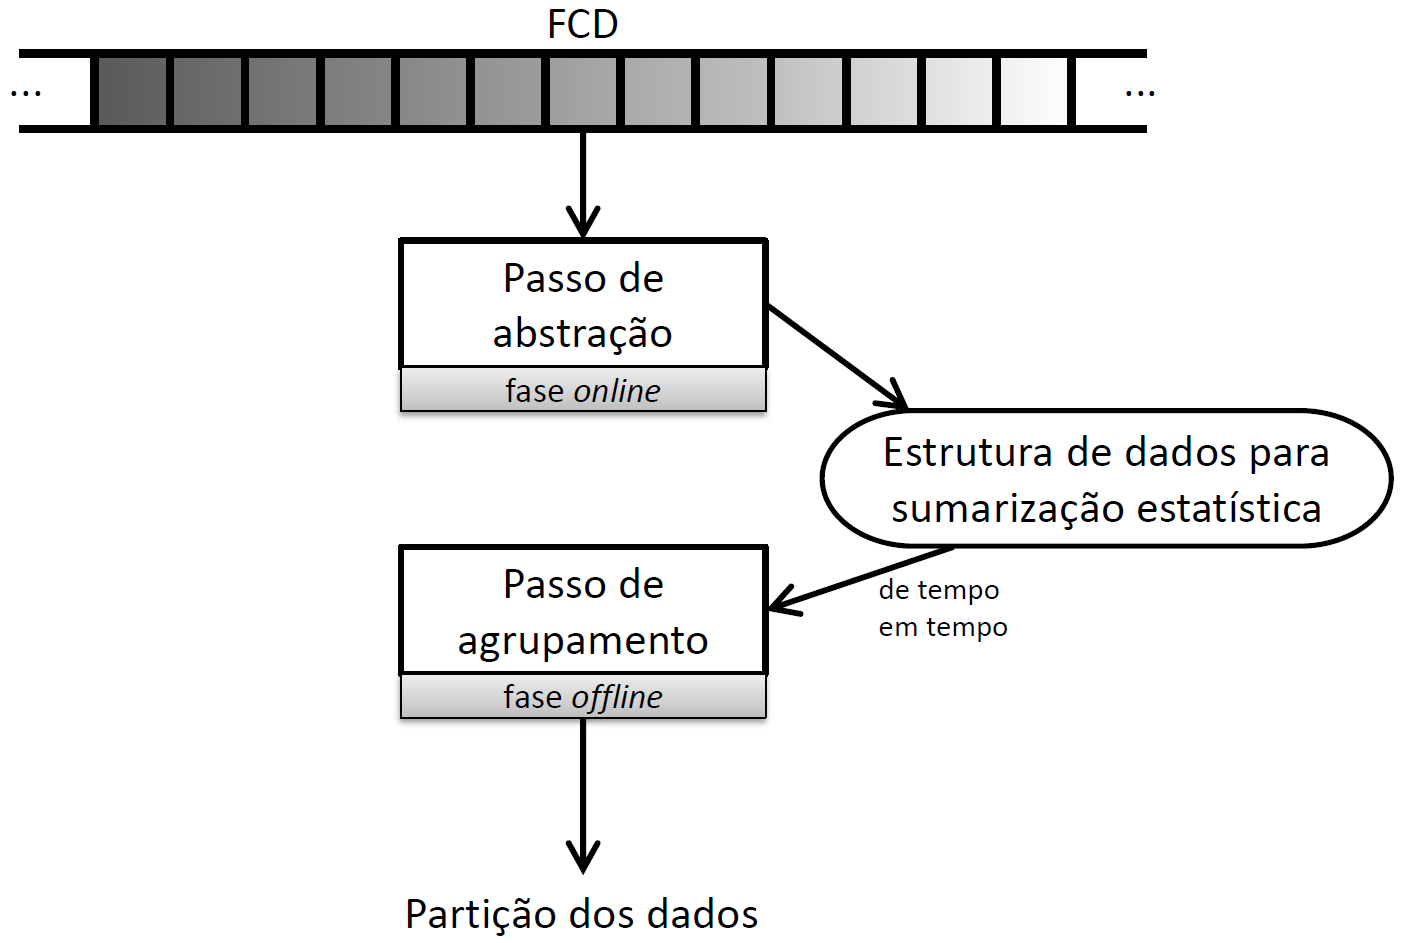
\includegraphics[width=0.7\textwidth]{figures/onlineOffline}
	\caption{\emph{Framework} \emph{online-offline} \cite{Silva2013}}\label{Fig:onlineOffline}
\end{figure}

A fase \emph{online}, abstração dos dados, sumariza os dados do FD com o auxílio de estruturas particulares para lidar com restrições de espaço e memória das aplicações FD. Essas estruturas de sumarizam os dados para preservar o significado dos objetos originais sem a necessidade de armazená-los. Estruturas frequentemente utilizadas são vetores de atributos, arranjos de protótipos e grades de dados. Essas estruturas são melhor detalhadas na \autoref{chConceitos:FD:Sumario}.

Para a contínua sumarização dos exemplos que chegam e dar maior importância aos exemplos mais recentes, uma abordagem popular é a definição de janelas temporais, como apresentado na \autoref{chConceitos:FD:Janelas}.

Durante o passo de abstração, algoritmos de agrupamento em FD devem utilizar mecanismos para detecção de \emph{outliers} que sejam capazes de diferenciar verdadeiros \emph{outliers} de evolução de grupos (\autoref{chConceitos:FD:Desvios}), uma vez que a distribuição dos dados pode variar de acordo com o tempo.

Na fase \emph{offline} é possível obter uma partição dos dados pelo passo de agrupamento. Neste momento, pode ser necessária a definição de alguns valores de entrada (número de grupos, por exemplo) para que seja possível ter uma visão geral dos grupos do FD. Algoritmos de agrupamento tradicionais podem ser utilizados considerando o conjunto de estruturas de sumarização para encontrar uma partição dos dados. O formato dos grupos encontrados está ligado ao algoritmo de agrupamento empregado, por exemplo, o $k$-\emph{means} \cite{macqueen1967} gera grupos hiperesféricos enquanto o DBSCAN \cite{Ester1996} é capaz de descobrir grupos de formatos aleatórios.

O \emph{framework} apresentado nesta seção é frequentemente utilizado para o desenvolvimento de novas técnicas de agrupamento em FD. Algumas dessas propostas são discutidas no \autoref{ChSemi}.